\documentclass[adraft, copyright, creativecommons]{eptcs} % TODO: Change to submission at the end
\providecommand{\event}{TERMGRAPH 2022} % Name of the event you are submitting to
% \usepackage{breakurl}             % Not needed if you use pdflatex only.
\usepackage{underscore}           % Only needed if you use pdflatex.

% My packages
\usepackage{orcidlink} % Orcid links
\newcommand\Mark[1]{\textsuperscript#1}

\usepackage{amssymb} % \square command
% Footnotes inside tables
\usepackage{footnote}
\usepackage{glossaries} % Glossary
\makesavenoteenv{tabular}
\makesavenoteenv{table}
\usepackage[nameinlink]{cleveref} % Reference footnotes.
\crefname{figure}{{figure}}{figures}
\Crefname{figure}{{Figure}}{Figures}
\crefformat{footnote}{#2\footnotemark[#1]#3}
% Math
\newtheorem{definition}{Definition}
\newcommand{\definitionautorefname}{Definition}
% Acronyms
\newacronym{bpmn}{BPMN}{Business Process Modeling Notation}

\title{BPMN semantics formalization and \\ model checking using graph grammars}
\author{Tim Kräuter\Mark{*}\orcidlink{0000-0003-1795-0611}, \quad
Harald König\Mark{\textdagger}\Mark{*}\orcidlink{0000-0001-6304-6311}, \quad
Adrian Rutle\Mark{*}\orcidlink{0000-0002-4158-1644}, \quad
Yngve Lamo\Mark{*}\orcidlink{0000-0001-9196-1779}
\institute{
\Mark{*}Western Norway University of Applied Sciences, Bergen, Norway
}
\institute{
\Mark{\textdagger}University of Applied Sciences, FHDW, Hannover, Germany}
\email{tkra@hvl.no, harald.koenig@fhdw.de, aru@hvl.no, yla@hvl.no}
}
\def\titlerunning{BPMN semantics formalization and model checking using graph grammars}
\def\authorrunning{Kräuter \textit{et al.}}
\begin{document}
\maketitle

% Maximum 8 pages for the first extended abstract!
% At the end, 15 pages for the proceedings.

% TODO: Semantics vs. execution semantics?
% process snapshot vs. process instance

\begin{abstract}
The BPMN is a widely used standard notation to define intra- and inter-organizational workflows to improve the communication between domain experts and software developers.
However, the informal textual description of the BPMN execution semantics hinders BPMN from reaching its full potential since BPMN constructs are interpreted differently, and behavioral properties cannot be checked.
Consequently, we propose a formalization of the BPMN execution semantics based on a model transformation to graph grammars.
The formalization is one of the most complete regarding supported BPMN constructs and enables model checking of BPMN-specific and custom properties.
Moreover, we implemented our approach and made the resulting tool accessible on the web.
\end{abstract}

\section{Introduction}
% \begin{itemize}
%     \item State goals: Semantics formalization and reference implementation (more/other constructs supported than recent approaches)
% \end{itemize}

% Short Motivation: Formalization of the natural language semantics and model checking
The \gls*{bpmn} is a widely used standard notation to define intra- and inter-organizational workflows to improve the communication between domain experts and software developers.
However, the informal textual description of the BPMN execution semantics hinders its full adoption \cite{objectmanagementgroupBusinessProcessModel2013, corradiniFormalApproachAnalysis2021}.
Consequently, to develop BPMN's full potential, we propose a new approach to formalize the BPMN execution semantics based on graph grammars.
The formalization in our approach is one of the most complete regarding supported BPMN constructs and enables model checking of BPMN-specific and custom properties.

The approach is summarized as a BPMN process model in \cref{fig:approach}.
It is based on a model transformation from BPMN process models to graph grammars.
Thus, our approach is \textit{generative}, i.e., it constructs a new graph grammar including rules and a start graph for each BPMN process model.
This is a major difference compared to other approaches such as \cite{corradiniFormalApproachAnalysis2021, vangorpVisualTokenbasedFormalization2013}, where only the BPMN process model is parsed, but the rewrite rules are fixed.

\begin{figure}[h]
    \centering
    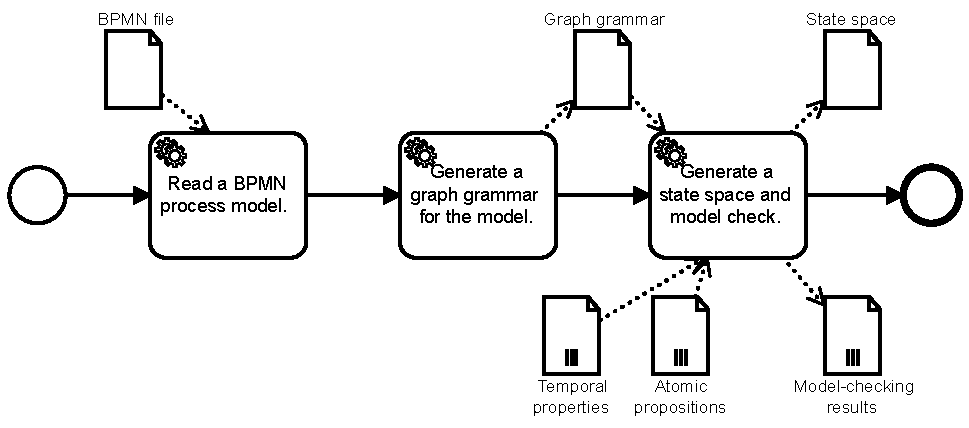
\includegraphics[width=0.55\textwidth]{images/full-approach.pdf}
    \caption{Overview of the proposed approach}
    \label{fig:approach}
\end{figure}

% Paper outline
The remainder of this paper is structured as follows.
First, we describe the semantics formalization using graph grammars in detail (\cref{sec:formalization}) before explaining how this can be utilized for model checking BPMN-specific and custom properties (\cref{sec:modelChecking}).
Second, we shortly present the implementation of our approach resulting in a web-based tool.
Finally, we discuss related work regarding BPMN feature coverage in \cref{sec:relatedWork} and conclude in \cref{sec:conclusion}.

\section{Semantics formalization} \label{sec:formalization}

Since our approach is a model transformation from BPMN to graph grammars it will generate a \emph{start graph} and \emph{production rules} for a given BPMN process model.
However, we do not support all possible BPMN models.
\Cref{fig:bpmnConstructsOverview} depicts the BPMN constructs supported by our approach.
We compare the extent of our formalization to other approaches later in this paper.

\begin{figure}[h]
    \centering
    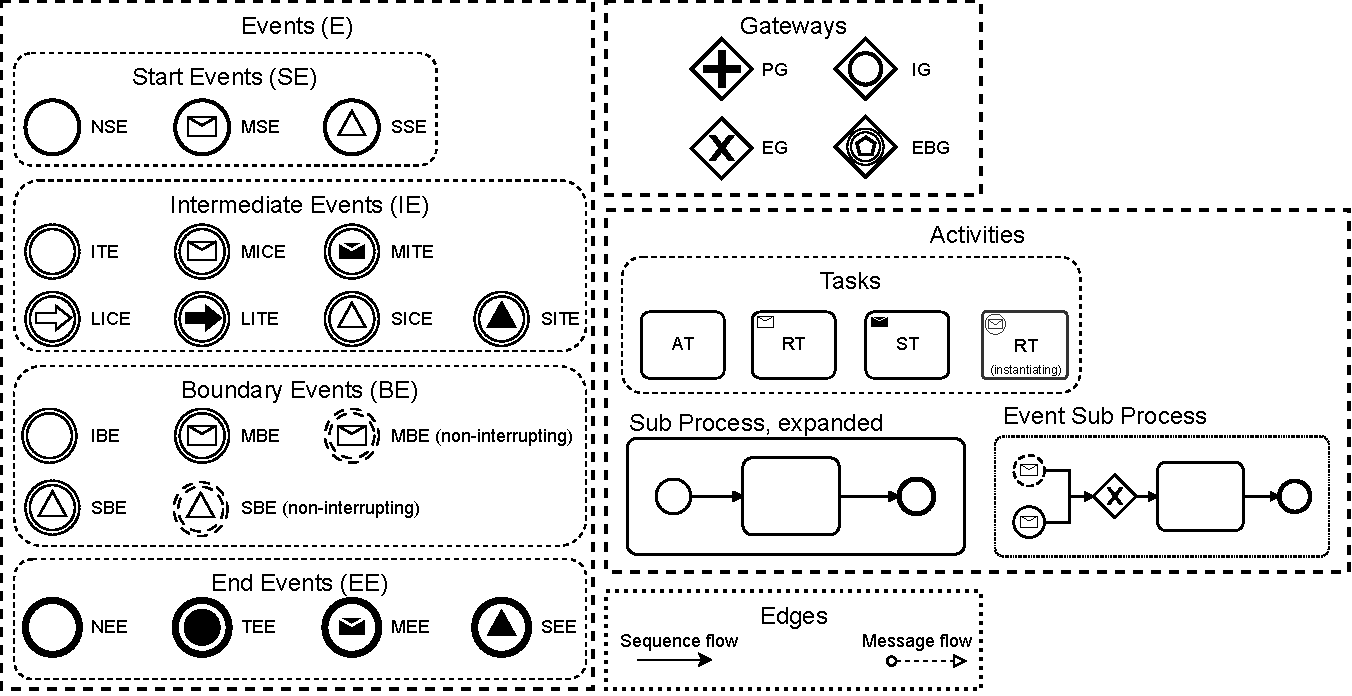
\includegraphics[width=0.8\textwidth]{images/bpmn_semantics-feature_overview.pdf}
    \caption{Overview of the supported BPMN constructs (structure adapted from \cite{houhouFirstOrderLogicVerification2022})}
    \label{fig:bpmnConstructsOverview}
\end{figure}

Our graph-transformation semantics are token-based as in the informal description of the BPMN specification \cite{objectmanagementgroupBusinessProcessModel2013}.
Thus, to describe processes holding tokens during execution we use the type graph shown in \cref{fig:typeGraph}.
The type graph is depicted using a UML class diagram-like syntax.

\begin{figure}[h]
    \centering
    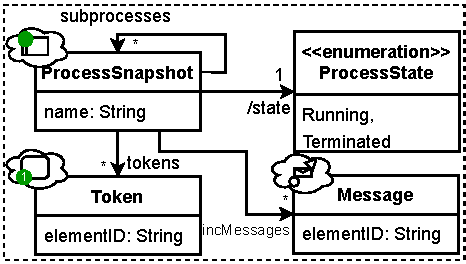
\includegraphics[width=0.5\textwidth]{images/bpmn_semantics-typegraph.pdf}
    \caption{BPMN execution type graph}
    \label{fig:typeGraph}
\end{figure}

We use \textsf{ProcessSnapshot} to denote a running BPMN process with a certain token distribution since it describes one state in the history of process states during the execution.
Every \textsf{ProcessSnapshot} has a set of \textsf{tokens} and \textsf{subprocesses}.
A \textsf{ProcessSnapshot} has the state \textsf{Terminated} if it has no \textsf{tokens} or \textsf{subprocesses}, else it has the state \textsf{Running}.
Using this type graph we can now define how the start graph and graph-transformation rules for the different BPMN constructs are created.
% TODO: Describe that we just work on tokens.
% TODO: Describe what the token position is.

% How is a start graph generated?
The generation of the start graph for a BPMN model is straightforward.
For each pool in the BPMN model we generate a process snapshot, if the pool contains a none start event (NSE).
A BPMN pool is depicted as a vertical lane with a name on the left and contains BPMN elements.
For each NSE we add a token to the respective process snapshot.
Furthermore, we consider to allow the user to define a start graph similar to how he could define atomic propositions for custom properties (see \cref{subsec:customProperties}).

We will now describe the rule generation for some selected elements to give a brief overview how the model transformation to graph grammars works.
\subsection{Activities}
% Task with implicit exclusive and parallel gateways.
% TODO: Describe this and draw parallels to gateways
\begin{figure}[h]
    \centering
    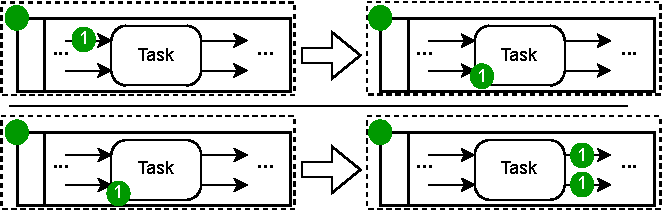
\includegraphics[width=0.5\textwidth]{images/bpmn_semantics-task-rules.pdf}
    \caption{Rules for a task with two incoming and outgoing sequence flows.}
    \label{fig:taskRules}
\end{figure}

\subsection{Events}
% TODO: Describe message Events and maybe draw parallels to other events.

\subsection{Process termination}
Process termination is implemented using a general rule, applicable to all process snapshots.
The rule is automatically generated once during the model transformation to graph grammars and is used to terminate processes, sub processes and event sub processes.
It uses non-application conditions to forbid tokens and sub processes for a process snapshot and then change its state from running to terminated\footnote{The terminate rule implemented in Groove is contained in the artifacts of this paper \cite{timkrauterArtifactsTERMGRAPH2022}.}.

\section{Model checking BPMN} \label{sec:modelChecking}

Model-checking a BPMN process model is straightforward after a graph grammar describing its execution semantics has been generated.
\Cref{fig:approach} depicts the inputs and outputs of model checking.

Besides a graph grammar, a set of temporal properties to be checked and the atomic propositions used in the properties must be supplied.
Atomic propositions are formalized as graph conditions that can match a state in the state space.
An atomic proposition holds in a state if and only if the graph associated with the atomic proposition is a subgraph of the graph associated with the state. % Cite groove/Rensink here.
This enables model checking of temporal properties using the defined atomic propositions.

Similar to other work, we differentiate between \emph{BPMN-specific properties} defined generally for all BPMN process models and \emph{custom properties} tailored towards a particular BPMN process model.
We will now give an example of two predefined BPMN-specific properties and how they can be checked using our approach.
Then, we describe how custom properties can be constructed and checked.

\subsection{BPMN-specific properties}
Two BPMN-specific behavioral properties, namely, Safeness and Soundness, are defined in \cite{corradiniClassificationBPMNCollaborations2018}.
Soundness is further decomposed into (i) \emph{Option to complete}: any running process instance must eventually complete, (ii) \emph{Proper completion}: at the moment of completion, each token of the process instance must be in a different end event, (iii) \emph{No dead activities}: any activity can be executed in at least one process instance \cite{corradiniClassificationBPMNCollaborations2018}.
We do not consider structural properties since they can be checked using a standard process modeling tool without implementing execution semantics.
As an example, we will now describe how to implement the \emph{Safeness} and \emph{Option to complete} properties using graph transformations.

% Safe
A BPMN process model is \emph{safe} if during its execution at most one token occurs along the same sequence flow \cite{corradiniClassificationBPMNCollaborations2018}.
\emph{Safeness} is checked in our implementation using the LTL property defined in \eqref{eq:safeness}.
The atomic property \textsf{Unsafe} is true if and only if two tokens of one process snapshot have the same position\footnote{\label{footnote:atomicProps}Groove rules for the atomic properties \textsf{Unsafe} and \textsf{AllTerminated} are contained in the artifacts of this paper \cite{timkrauterArtifactsTERMGRAPH2022}.}.

\begin{align}
    & \square (\neg \,\text{Unsafe}) \label{eq:safeness} \\
    \lozenge (& \square(\text{AllTerminated})) \label{eq:optionToComplete}
\end{align}

% Option to complete
\emph{Option to complete} is checked in our implementation using the LTL property defined in \eqref{eq:optionToComplete}.
The atomic property \textsf{AllTerminated} is true if and only if there exists no process snapshot in the state running, i.e., all process snapshots are terminated\cref{footnote:atomicProps}.

Both properties can be checked using our implementation \cite{timkrauterArtifactsTERMGRAPH2022}.
To fully check Soundness, the proper completion and no dead activities properties must be checked.
The information needed to check these properties is present in the generated state space, such that checking these properties is possible manually and can be automatized in the future.
\subsection{Custom properties} \label{subsec:customProperties}
% Custom LTL properties

% Defining atomic propositions in BPMN is a novelty.
To make model checking user-friendly, we let users define atomic propositions in the BPMN syntax.
BPMN is usually explained and formalized using tokens, which flow through the process model.
Thus, to define an atomic proposition, we let the user attach tokens to his BPMN process model, which we can automatically convert to a graph condition.

For example, the token distribution shown in \cref{fig:atomicProposition} defines two running process instances with a token in task A.
Differently colored tokens define different process instances.
Thus, a user must not be aware of the graph transformation semantics used for execution.
This leads to a significant advantage compared to currently implemented approaches, which can be adapted even when not using graph transformations.

\begin{figure}[h]
    \centering
    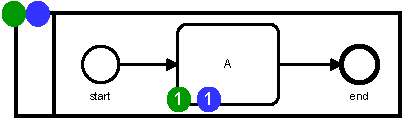
\includegraphics[width=0.3\textwidth]{images/bpmn_semantics-atomicProp.pdf}
    \caption{Token distribution defining an atomic proposition.}
    \label{fig:atomicProposition}
\end{figure}

The token visualization was significantly inspired by the excellent bpmn-js-token-simulation\footnote{\url{https://github.com/bpmn-io/bpmn-js-token-simulation}}.
\section{Implementation} \label{sec:impl}
% Tool
\Cref{fig:implScreenshot} depicts a screenshot of the implemented tool.
The tool is open-source, publicly available, and does not require any installation \cite{timkrauterArtifactsTERMGRAPH2022}.

\begin{figure}[h]
    \centering
    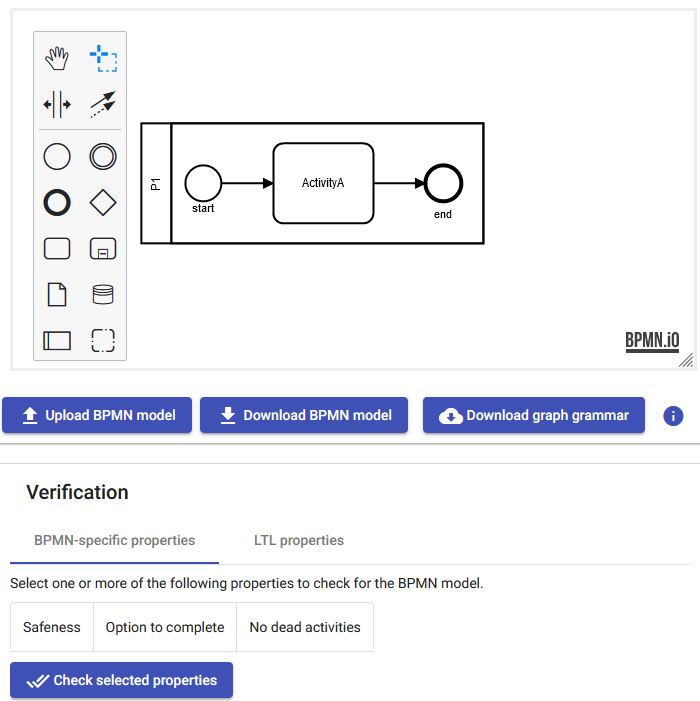
\includegraphics[width=0.6\textwidth]{images/impl.png}
    \caption{Screenshot of the web interface of the tool}
    \label{fig:implScreenshot}
\end{figure}

The tool implements the approach depicted in \cref{fig:approach}.
We are using the graph-transformation tool Groove\footnote{\url{https://groove.ewi.utwente.nl/about}} in our implementation \cite{ghamarianModellingAnalysisUsing2012} since it supports all the theoretical constructs that we need.

% Evaluation
To evaluate the correctness of our implementation, we created a comprehensive test suite, which verifies correct rule generation for the implemented BPMN constructs \cite{timkrauterArtifactsTERMGRAPH2022}.

\section{Related work} \label{sec:relatedWork}
% Van gorp
A BPMN formalization based on in-place graph transformation rules is given in \cite{vangorpVisualTokenbasedFormalization2013}.
The formalization covers a substantial part of the BPMN specification, including complex concepts such as inclusive gateway merge and compensation.
In addition, graph transformation rules are visual and thus can easily be matched to the informal description of the execution semantics in the specification \cite{objectmanagementgroupBusinessProcessModel2013}.
The graph transformation rules were implemented in a prototype using GrGen.NET.
Unfortunately, the implementation is not publicly accessible anymore.
Moreover, they do not support model checking since their goal is formalization.

% BProve/Corradini
The tool BProVe\footnote{\url{http://pros.unicam.it/bprove/}} is based on formal BPMN semantics given in rewriting logic and implemented in the Maude system.
Using these semantics, BProVe enables the verification of custom temporal properties for process models.
Furthermore, the tool is easily accessible online and includes checking of BPMN-specific properties, such as safeness and soundness \cite{corradiniFormalApproachAnalysis2021}.
They also support checking custom LTL properties.

% fbpmn/Houhou
The verification framework \textsf{fbpmn} uses first-order logic to formalize and check BPMN process models \cite{houhouFirstOrderLogicVerification2022}.
This formalization is then realized in the TLA\textsuperscript{+} formal language and can be model-checked using TLC.
Their framework and related information is open source and freely available online\footnote{\url{https://github.com/pascalpoizat/fbpmn}}.
Similar to BProVe, \textsf{fbpmn} allows checking BPMN-specific properties, such as safeness and soundness.
However, they do not allow a user to define custom temporal properties.

Besides these three approaches, there are many more BPMN formalizations, for example, based on Petri Nets \cite{dijkmanSemanticsAnalysisBusiness2008} or process algebras \cite{wongProcessSemanticsBPMN2008}.
We looked in detail at these three approaches since they support a significant subset of the BPMN constructs, have easily accessible and well-documented tool support, and are pretty recent.

Nevertheless, different approaches support a different subset of the BPMN constructs, which impacts their usefulness in practical scenarios.
\Cref{tab:supportedconstructs} depicts which BPMN constructs are supported by the different approaches compared to our approach.

\begin{table}[htbp]
    \caption{Constructs supported by different BPMN formalizations (overview based on \cite{vangorpVisualTokenbasedFormalization2013}).}
    \label{tab:supportedconstructs}
    \begin{tabular}{l l l l l}
    \hline
      Feature & Van Gorp &  Corradini & Houhou & This\\
      & et al. \cite{vangorpVisualTokenbasedFormalization2013} & et al. \cite{corradiniFormalApproachAnalysis2021}& et al. \cite{houhouFirstOrderLogicVerification2022} & paper\\
      \hline
      \textit{Instantiation and termination} & &\\
      Start event instantiation & X & X & X & X\\
      Exclusive event-based gateway instantiation & X & & & X\\
      Parallel event-based gateway instantiation &  & & & \\
      Receive task instantiation & & & & X\\
      Normal process completion & X & X & X & X\\
      \textit{Activities} & & & &\\
      Activity & X & X & X & X\\
      Subprocess & X & X* & X & X\\
      Ad-hoc subprocesses & & & &\\
      Loop activity & X & & &\\
      Multiple instance activity & & & & \\
      \textit{Gateways} & & & &\\
      Parallel gateway & X & X & X & X\\
      Exclusive gateway & X & X & X & X\\
      Inclusive gateway (split) & X & X & X & X\\
      Inclusive gateway (merge) & X & & X & X\\
      Event-based gateway &  & X\footnote{Does not support receive tasks after event-based gateways.} & X & X\\ % No timer and conditional events after event based gateway supported.
      Complex gateway & & & &\\
      \textit{Events} & & & & \\
      None Events & X & X & X & X\\
      Message events & X & X & X & X\\
      Timer Events & & & X & \\
      Escalation Events & & & & \\
      Error Events (catch) & X & & &\\
      Error Events (throw) & X & & &\\
      Cancel Events & X & & &\\
      Compensation Events & X & & &\\
      Conditional Events & & & &\\
      Link Events & X & & & X\\
      Signal Events & X & & & X\\
      Multiple Events &  & & & \\
      Terminate Events & X & X & X & X\\
     Boundary Events & X\footnote{Only supports interrupting boundary events on tasks.} & & X\footnote{Only supports message and timer events.} & X\\ % To the same extent as the event support
      Event subprocess &  &  &  & X\\
    \end{tabular}
\end{table}

% Summarize the findings and explain them in more detail
% Explain Van Gorp in detail
Van Gorp et al. \cite{vangorpVisualTokenbasedFormalization2013} cover a large part of the BPMN semantics.
However, they do not support Event-based gateways and event subprocesses, while their support for boundary events is minimal.
Especially, Event-based gateways are often used and supported by every other approach.

% Explain Corradini in detail
Corradini et al. \cite{corradiniFormalApproachAnalysis2021} does only support message and terminate events.
However, many other types of events exist and are used in practice.
Moreover, they do not support the occurrence of receive tasks after Event-based gateways.
Nevertheless, the same behavior can be achieved using message events.
% Limited subprocess support?
% Explain Houhou in detail
In addition to \cite{corradiniFormalApproachAnalysis2021}, Houhou et al. \cite{houhouFirstOrderLogicVerification2022} support timer and the use of message and timer events as both interrupting and non-interrupting boundary events.
However, the support of different event types remains limited compared to \cite{vangorpVisualTokenbasedFormalization2013}.

% Our semantics is the only one that generates "rules" and not only converts the model to some representation, right?. So we are higher-order?
Besides semantics, our approach is also unique since it not only transforms a BPMN process model into a different representation but also generates graph-transformation rules for this specific model.
Other approaches, for example, rely on a fixed generic set of rules \cite{vangorpVisualTokenbasedFormalization2013} or Maude implementation \cite{corradiniFormalApproachAnalysis2021}.
% What about Houhou?
\section{Conclusion \& future work} \label{sec:conclusion}
% Summary

% Formalization
% Model checking
% Tool

% Future work
We aim to improve our formalization and resulting tool in multiple ways in the future.
% More semantics
First, we intend to extend our formalization to support even more BPMN constructs for example error, cancel and compensation events.
% Proper evaluation
Second, we plan to evaluate our approach on syntactical models and on models from open repositories such as the "BPM Academic Initiative Model Collection" \cite{weskeModelCollectionBusiness2020} and "Camunda BPMN for
Research"\footnote{\url{https://github.com/camunda/bpmn-for-research}}.
% Implementing the atomic proposition definition
Third, we want to extend the features of our tool.
One should be able to define atomic propositions for model checking in the tool directly, as described in \cref{sec:modelChecking}.
% Counterexample simulation similar to Houhou
Furthermore, counterexamples found during model checking should be visualized directly in the tool, similar to the implementation in \cite{houhouFirstOrderLogicVerification2022}, such that users must not be aware of the underlying implementation in Groove.
% Automatize more BPMN-specific properties
Finally, we aim to directly integrate \emph{Soundness} as an BPMN-specific property together with its sub-properties \emph{Proper completion} and \emph{No dead activities} into the tool \cite{corradiniClassificationBPMNCollaborations2018}.
\bibliographystyle{eptcs}
\bibliography{bib} % TODO: Should be bib.
\end{document}
